\chapter{Results}\label{chapter:results}

This chapter details the results from all the tests in the previous chapter. It
also details whether the system as a whole has satisfied the project assignment.

\todo{Results of all functional tests, following the functional requirements have to be mentioned here}

\clearpage
\section{Test Results}

%The below input is a subsection of the above section

\subsection{FPGA Simulation Results}
While testing \textit{ChaosM} with the aim of accomplishing FR3
some problems were encountered. These tests show post-route simulation on our
toplevel vhdl design. This includes the ebi controller, clock controller and the pipeline(s).
The tests looked like this:

\begin{itemize}
\item Load a program into the processors’ instruction memory. The program will load from its input buffer and store to its output buffer.\\
\item Load input into the first core’s input buffer. The data loaded was “BEEF” for the first pipeline and “1EEF” for the second pipeline (if applicable).\\
\item Read the result from the last core output buffer. The result can be read from the signal called “EBI data”.\\
\end{itemize}


\paragraph{First Test}

The first test was one pipeline with four cores. The timing simulation of this
test is  shown in Figure \ref{fig:one_pipe_four_core}. As the Figure shows,
the simulation outputs the correct results shown by signal in orange at the
point  marked by the yellow, vertical line.

\begin{figure}[H]
    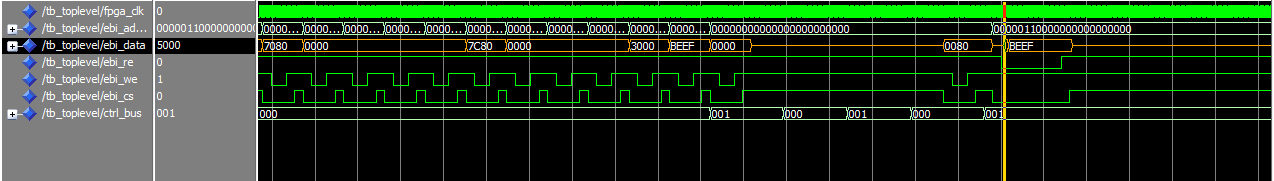
\includegraphics[width=1.3\textwidth]{figures/fpga/result_1_pipe_4_cores.PNG}
    \caption{Result from timing simulation of one pipeline with four cores.}
    \label{fig:one_pipe_four_core}
\end{figure}

\paragraph{Second Test}
The second test was two pipelines with four cores in each. The timing simulation
of this test did not work as expected. Out of the two pipelines simulated only one
gave correct results, see Figure \ref{fig:two_pipe_four_core}. The first core
outputted only zeros, as the yellow line shows,  while the second pipeline outputted the correct result “1EEF”.

\begin{figure}[H]
    \centering
    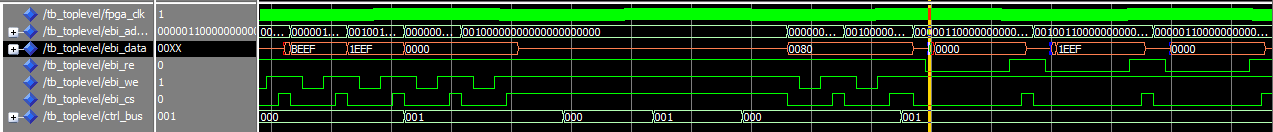
\includegraphics[width=1.3\textwidth]{figures/fpga/result_2_pipe_4_cores.PNG}
    \caption{Result from timing simulation of two pipelines with four cores each.}
    \label{fig:two_pipe_four_core}
\end{figure}


\subsection{FPGA Configuration Results}
Even though one pipeline with four cores simulated correctly in ModelSim, the configured FPGA
did not work as in the simulation. It behaved nondeterministically with little to no pattern
in the outputted results. A lot of debugging was done and it seems as though the problems
lie in the communication between the microcontroller and the FPGA.




\clearpage
% !TEX root = ../../report.tex
\section{Power Measurements}

Since this is the report of the energy efficiency group, all components of
system the have been chosen with energy efficiency in mind. In order to measure
the efficiency of our design decisions, a set of power measurements were
performed. This section outlines the results of those measurements.

\begin{table}
    \begin{tabular}{lllll}
	State & FPGA                         & Audio source & Sense3v3 & Sense1v8 \\
	\hline \\
	A     & Idle                         & -            & 140mA    & 75mA \\
	B     & Computational simple filters & ADC          & -        & - \\
	C     & Computational heavy filters  & ADC          & -        & - \\
        D     & Computational simple filters & SD-card      & -        & - \\
        E     & Computational heavy filters  & SD-card      & -        & -
    \end{tabular}
    \label{tab:results/power-measurement}
    \caption{FILL OUT CAPTION}
\end{table}

\todo{Preliminary results, will be fleshed out once we have a running system}


\clearpage
\subsubsection{Power comparision using energy profiling}

An important feature included with Simplicity Studio and Silicon Labs microcontrollers
is the possibility to easily monitor the power consumption on the running system.
This allows for easier development of energy efficient code, and can help
with finding and tracing down bugs. 
This is a feature called \textit{energyAware Profiler}, and it is thoroughly 
described in Silicon Labs application note \cite{energydbg}.

Most of the code used in this project is already based on highly optimized 
examples with respect to energy efficiency.
The example provided by Silicon Labs named {\bf preamp} is comparable to the main
DMA dataflow, as their net work is similar. Both program uses DMA and moves samples 
from ADC to DAC. The difference is that the non-example code includes deinterleaving
and interleaving of the audio channels. Refere to section \ref{} for details. Figures \ref{fig:fpga} and \ref{fig:preamp}
shows the energy consumption by the Microprocessor when running each program.

\FloatBarrier
\chapter{FPGA}\label{chapter:fpga}

As this project requires us to implement a MIMD processor in VHDL, we realized
our design through implementing it in VHDL, and running the final processor on a
Spartan-6\cite{fpga-chip} FieldProgrammableGateArray.

Our MIMD processor design is was realized through pipelined cores connected
sequentially in a pipeline of their own. Since the processor consists of
homogenous cores, each core can receive and run the same instructions. To
realize this as a ``Multiple Instructions, Multiple Data'' (``MIMD''), the first
core in the sequential core-pipeline is the only one which can work with the
data given to said pipeline by the EBI bus. The next core then works on the
output of the first core, and in this fashion each core in the pipeline works on
its own data independently of the data any other core is currently working
on\footnote{This is how we realize the ``Multiple Data'' part of the MIMD
definition.}.

And each of the processor cores has its own instruction memory, so that they can
run each their own instructions, and that's how we have realized the ``Multiple
Instruction'' part of the MIMD definition.
\newpage
\FloatBarrier
\section{Design Planning}\label{section:fpga-design}
\subsection{Design start}

As soon as it became decided that our project was going to aim for producing
some kind of ``sound-effect manipulating processor'', the group started looking
into how sound-effects were actually accomplished.

It quickly became apparent that for the most common, as well as the more
complicated effects, Fourier-transforms were crucial to the sound-manipulation
process. At least when sound manipulation was intended to run quickly enough,
as well as successfully on a computer processor.

This represented an (until now) unforeseen problem: Fourier-transforms are
algorithmically heavy in both time complexity and storage-space complexity,
which has the consequence that we would have to devote more of the FPGA
resources into circuits which could handle something as intensive as a
Fourier-transform. Especially if we wanted to perform these sound-effects in
real-time.

In effect, this revelation forced us to from a very early point to be
concerned about resource management on the FPGA.

\subsection{Fourier-transforms}\label{subsection:fpga-design-ft}

Looking into which types of Fourier-transform algorithms we could use on an
embedded device, in a manner as efficiently as possible, and yet real-time,
we ended up looking at Sliding-Discrete-Fourier-Transforms\cite{SD-FT} (or more
colloquially known as SD-FTs\footnote{This is discussed in more detail in
section \ref{subsubsection:fpga-alu-ft}.}).
\missingfigure{Maybe insert a figure here showing how the SD-FT works on each
sample at a time?}

This Fourier-transform would enable the FPGA to receive a live stream of
data samples representing sound from an input device through a mini-jack on the
PCB, or just from the DMAs of the MCU if the input was a file on a SD-card. And
then transform this live stream of samples into the frequency domain.

Since we now were able to work on each discrete sample while it was converted
into the frequency domain, we were now able to perform frequency based
sound-manipulations, such as basic high-pass and low-pass filters.

The sound-effect manipulations could now (in theory) be put to work.

\FloatBarrier
\subsection{Sequential processing cores?}\todo{Maybe find better subsection
title?}

Not all of the known sound-effects require (or are even possible) with a
Fourier-transform. Therefore it also became evident that for effects like say
the ``echo-effect'', we would need to do some post-processing after having
performed the inverse-Fourier-transform of the SD-FT\footnote{Sliding-Discrete
Fourier-transform, elaborated in the previous section
\ref{subsection:fpga-design-ft}.}.

Thus, so far this project required one processor-core to perform the SD-FT, and
another to perform the actual sound-effect done with the samples in the
frequency domain. A third core for the inverse SD-FT, and finally a fourth core
for any possible sound-manipulation that does not need a Fourier-transform (that
does not need to manipulate the data samples when converted into the frequency
domain).

With that reasoning in mind, we would need at least four processing cores, and
this for only one sound-channel. So for every additional sound-channel needed (
stereo needs two), we would have to add another four processor cores onto the
FPGA-chip.

It was decided early on to not settle for just one channel producing mono sound,
but to instead settle for at least two, so that we could listen to the output
on a stereo system. This let us then define the design for the processor
further, since it would need to have at the very least eight processor cores
implemented in some form of pipeline or other.

\subsection{Processing cores, 1-on-1}\todo{Maybe find better subsection title?}

Knowing we would need a minimum of eight processor cores on our FPGA processor,
and maybe more later down the line, we decided to start making things easier
for ourselves.

The decision was made to have all the cores homogenous, so that it would be
possible to send the same instructions to any core, being safe in the knowledge
that any core could perform said instructions.

This simplified the work in VHDL considerably, since we could then focus on
getting just \emph{one} processor core functioning, instead of say one
specifically for the SD-FT, another specifically tailored for the actual
sound-effects performed in the frequency domain, a third for the inverse-SD-FT,
and then the same as well for the fourth and final core performing the
``post-processing''. This would have (in all likelyhood) more than quadrupled
the amount of work required in VHDL for this project.

Due to all of the members in the FPGA-group taking the course TDT4255 \emph{
Computer Design} it may come as no surprise to any reader familiar with the
courses at IDI, NTNU, that this course was a big source of inspiration for the
development of our processor-core. Both the book\cite{tdt4255-book} and the
\emph{Computer Design} course were used as resources while developing the design
of this MIPS pipelined processor.

\subsection{Toplevel control register}\label{subsection:fpga-design-toplevel}


% !TEX root = ../../../report.tex
\FloatBarrier
\subsection{Audio Pipelines}\label{subsec:audio_pipelines}

\begin{figure}[H]
    \centering
    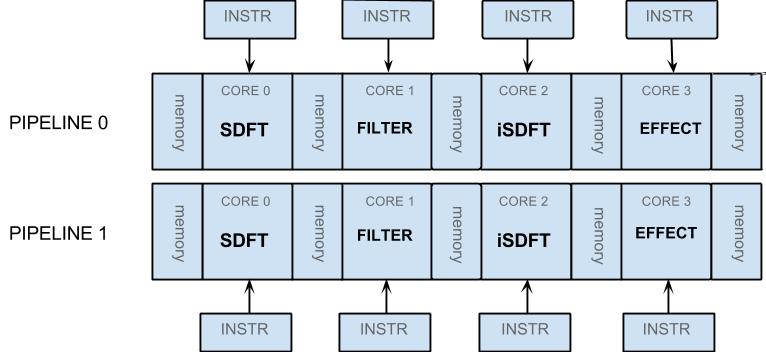
\includegraphics[height=150px]{figures/fpga/system_components_general_pipeline.png}
    \caption{Audio Pipeline Architecture}
    \label{fig:pipeline_architecture}
\end{figure}

\textit{ChaosM} consists of two audio processing pipelines, as illustrated in
Figure \ref{fig:pipeline_architecture}. These contain up to four processing cores
connected by data buffers. Each audio processing pipeline corresponds to one audio channel, operating on audio samples as elementary data elements.
The input/output frequency is directly tied to the sample rate of the input, which acts as a secondary clock input. The main system clock runs on the order of MHz, while this \textit{sample clk} is in the order of kHz and acts as a deadline for when new I/O is due.

\section{Processor Core}\label{section:fpga-processor-core}
\todo[inline]{How is the processor designed and \emph{why!}}

\input{chapters/fpga/processor-core/alu}

\subsection{Floating-point implementation design choices}

\subsection{Datapath/pipelining of the core}
\todo[inline]{Describe the pipelines of the cpu, and why it is implemented/
designed the way it is.}

\subsection{Memory access}
\todo[inline]{Why constant values go to the alu, and how it changes pipeline
layout. How the core accesses memory.}
\section{Internal memory\todo{Better title}}\label{section:fpga-internal-memory}
\todo[inline]{Should contain: Ringbuffer, Switch buffer, input/output buffers,
constant memory, inst memory, read and write lines to the fpga from the ARM.
Originally the ARM only needed access to the first and the last data buffer but
for debugging purposes the ARM was given access to all buffers.}
\todo[inline]{Short description? Discuss non-uniform memory access and important
things.}

\subsection{Intruction memory}
\todo[inline]{Describe the functionality and reasons behind decisions regarding
the instruction memory. -First revision done. Finished?}

The instruction memory for each core is how we realize the ``Multiple
Instructions'' part of the ``MIMD'' definition. This instruction memory which
each core has is how the separate cores can run each their own independent
instructions.

Due to the manner in which this system is intended to be intialized (as detailed
in section \ref{subsection:fpga-pipeline-startup}), another aspect of this
implementation choice is that before starting up all the cores (in effect
starting up the sequential pipelines), the MCU must through the EBI-bus write
the instructions into this instruction memory in each core, and in this manner
set up which core in the sequential pipelines is supposed to perform which job.

\subsection{Processor input/output memory}\label{subsection:fpga-internmem-IO}
\todo[inline]{Describe the need for memory to behave as both ringbuffer/queues,
and as switching buffers. Discuss why this is a good idea because of our
intended functionality, and how we utilize the FPGAs resources to implement it
in the best possible way.}

\subsection{Pipeline constant memory}
\todo[inline]{Why did we separate this from input/ouput memory? Why is it shared
between cores, and how? The reason we send it's values directly to the alu
instead of to the register file?}
\FloatBarrier
\section{Communication}

\subsection{The External Bus Interface}
The microcontroller communicates with the FPGA design using the External Bus
Interface (EBI) of the Giant Gecko microcontroller. The EBI is a parallel bus
with a separate data and address bus in addition to the chip select and read and
write enable signals, all active low\cite{efm_ebi}.

The communication between the MCU and the FPGA uses 23 address lines and 16
data lines. All transfers are initiated by the chip select signal going low.
Then, for write transfers, the data and address lines are set up and the
write enable signal is asserted, see figure \ref{fig:ebi_write}. For reads,
the address is set up and the data line is put in high impedance mode before
the read enable signal is asserted, see figure \ref{fig:ebi_read}.

\input{figures/fpga/communication-ebi-write}
\input{figures/fpga/communication-ebi-read}

\FloatBarrier
\subsection{The Internal Bus}

The internal bus is used to transfer data to and from modules in the FPGA.
All transfers are initiated by the microcontroller on the EBI bus, and the
EBI controller module translates between the EBI and the internal bus.

\subsubsection{The EBI controller}
The EBI controller module is used to handle EBI transfers initiated by the
microcontroller. It consists of a simple state machine, illustrated in
figure \ref{fig:ebi_ctrl_fsm}. When an EBI transfer is executed, the
internal bus, described in is used to store or retrieve data from a module
in the FPGA.

In the idle state, the EBI data lines are set as high impedance, which
causes the microcontroller to have control of the data bus. Only when
a value is read over the EBI bus, does the EBI controller take control of
the data lines.

To save power, a clock gate is used to turn off the functional clock to
the EBI controller when the chip select signal is deasserted.

\input{figures/fpga/communication-ebi-ctrl-fsm}

\subsubsection{Addressing}

Modules in the FPGA is addressed using a simple hierarchical scheme, where the
address is divided into three parts; the pipeline where the module is located,
the ``index'' of the module and an address specifying where in the module to
read or write data. Figure \ref{fig:ebi_addresses} illustrates the address
format.

\input{figures/fpga/communication-ebi-addresses}

\FloatBarrier
\subsubsection{Read Transfers}

A read transfer is initiated when the read enable line from the microcontroller goes low.
The EBI controller sets up the internal address signals and asserts the internal read enable
signal. This causes the requested data to be available in the next clock cycle. The EBI
controller switches to read state, where it remains until the read enable signal is deasserted.

\subsubsection{Write Transfers}

Write transfers are initiated the same way as read transfers. As the write-enable signal goes
low, the destination address is latched into the internal address bus and the internal data
lines are set to the value of the EBI data lines. The internal write enable signal is asserted
and the EBI controller enters the write state. In the write state the internal write enable
signal is reset, and when the EBI write enable signal is deasserted, idle mode is reentered.


% !TEX root = ../../../report.tex
\subsection{Instruction Set Architecture}\label{section:fpga-isa}

The processor was designed in a top-down fashion, starting with the instruction
set. The MIPS ISA used in the \textit{Computer
Design}\cite{tdt4255} course was a good starting point for the ISA used in this
project. In order to support as many different filters
and effects as possible, the processor supports all normal arithmetic
operations. Due to the requirements of doing Fourier transforms on the
processor, support for some floating point instructions was also included.

To make the decoding of instructions as easy as possible, instructions
were divided into three different instruction groups.

\subsubsection{Register-based Instructions}

The register-based instructions are instructions were both operands are
primarily registers. The group also includes a few instructions where
the second operand is an immediate value. The format of the
instructions are illustrated in Figure \ref{fig:regbased_instrs_format}. The
implemented functions can be found in Table \ref{tab:regbased_instrs}.

\input{figures/fpga/isa-regbased-format}
\FloatBarrier
\input{figures/fpga/isa-regbased-instructions}
\FloatBarrier

\subsubsection{Load Immediate Instruction}
The load immediate instruction is used to load an immediate constant into a
register. The format of the instruction can be found in figure
\ref{fig:ldi_format}. The value is loaded into register \texttt{\$r1}.

\input{figures/fpga/isa-ldi-format}
\FloatBarrier

\subsubsection{Branch Instruction}
The branch instruction checks condition flags and jumps accordingly. By
checking for various combinations of the condition flags, many different
conditions can be checked for. The format of the instruction is illustrated
in Figure \ref{fig:new_branch_format}.

\input{figures/fpga/isa-branch-format}
\FloatBarrier

\paragraph{Special Registers}

Due to the limited space in instruction words, only two registers at most can be
specified in an instruction. Some instructions, such as the load immediate and
load constant instructions do not specify any registers, only an immediate
offset constant.

The list of defined special registers can be found in Table \ref{tab:specregs}.

\input{figures/fpga/isa-special-registers}
\FloatBarrier

\section{Testing the FPGA}\label{section:fpga-testing}

\subsection{FPGA prototype}
\todo[inline]{How we tested that the FPGA was soldered onto the PCB. Can move this section.}

\subsection{Testing the processor design}
\todo[inline]{Testing methodology}

\subsection{Simulation}
\todo[inline]{Simluation description}

\subsubsection{Tests\todo{insert more of these, along with descriptions and reasons.}}

\subsection{Integrated tests}
\todo[inline]{Description of testing on board}

\subsubsection{Tests\todo{insert more of these, along with descriptions and reasons.}}




\begin{figure}[H]
    \centering
    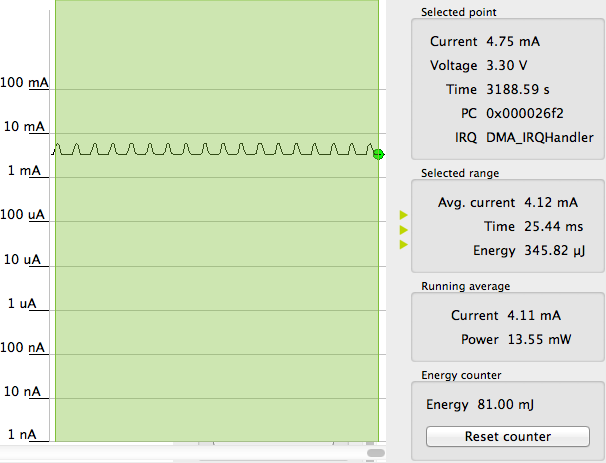
\includegraphics[width=250px]{figures/sw/preamp.png}
    \caption{Energy usage for demo code}
    \label{fig:preamp}
\end{figure}


As the figures suggests the energy consumption for each program are practically equal.


\clearpage
\section{Assignment results}

\todo[inline]{This is where we discuss the ``final'' state of the whole project.
Saying how it looks like, and what it can do beyond what was discussed in the
previous chapter.}

%The below input is a subsection of the above section
% !TEX root = ../../report.tex

\subsection{PCB Workarounds}

Due to the manual work involved in designing the PCB, and because it was fairly
unfamiliar ground for everyone involved, there were many things that could go
wrong. This section describes everything that was wrong with the PCB along with
what was done to fix it.

The first thing to happen was smoke appearing from the linear regulator upon
plugging in the power source. As it turned out, the footprint was mismatched
with the pinout of the component. The footprint had been fixed early on in the
process, but unfortunately the schematics had not been updated. The same turned
out to have happened with the low frequency crystal connected to the MCU.

Both of the above problems where solved by extra wiring. For the crystal, where
pin 1 and 4 was suppose to be used, pin 1 and 2 were used instead. As pins 2 and
3 were unconnected, a patch cable was soldered between pin 4 and 2.

\begin{figure}[H]
    \centering
    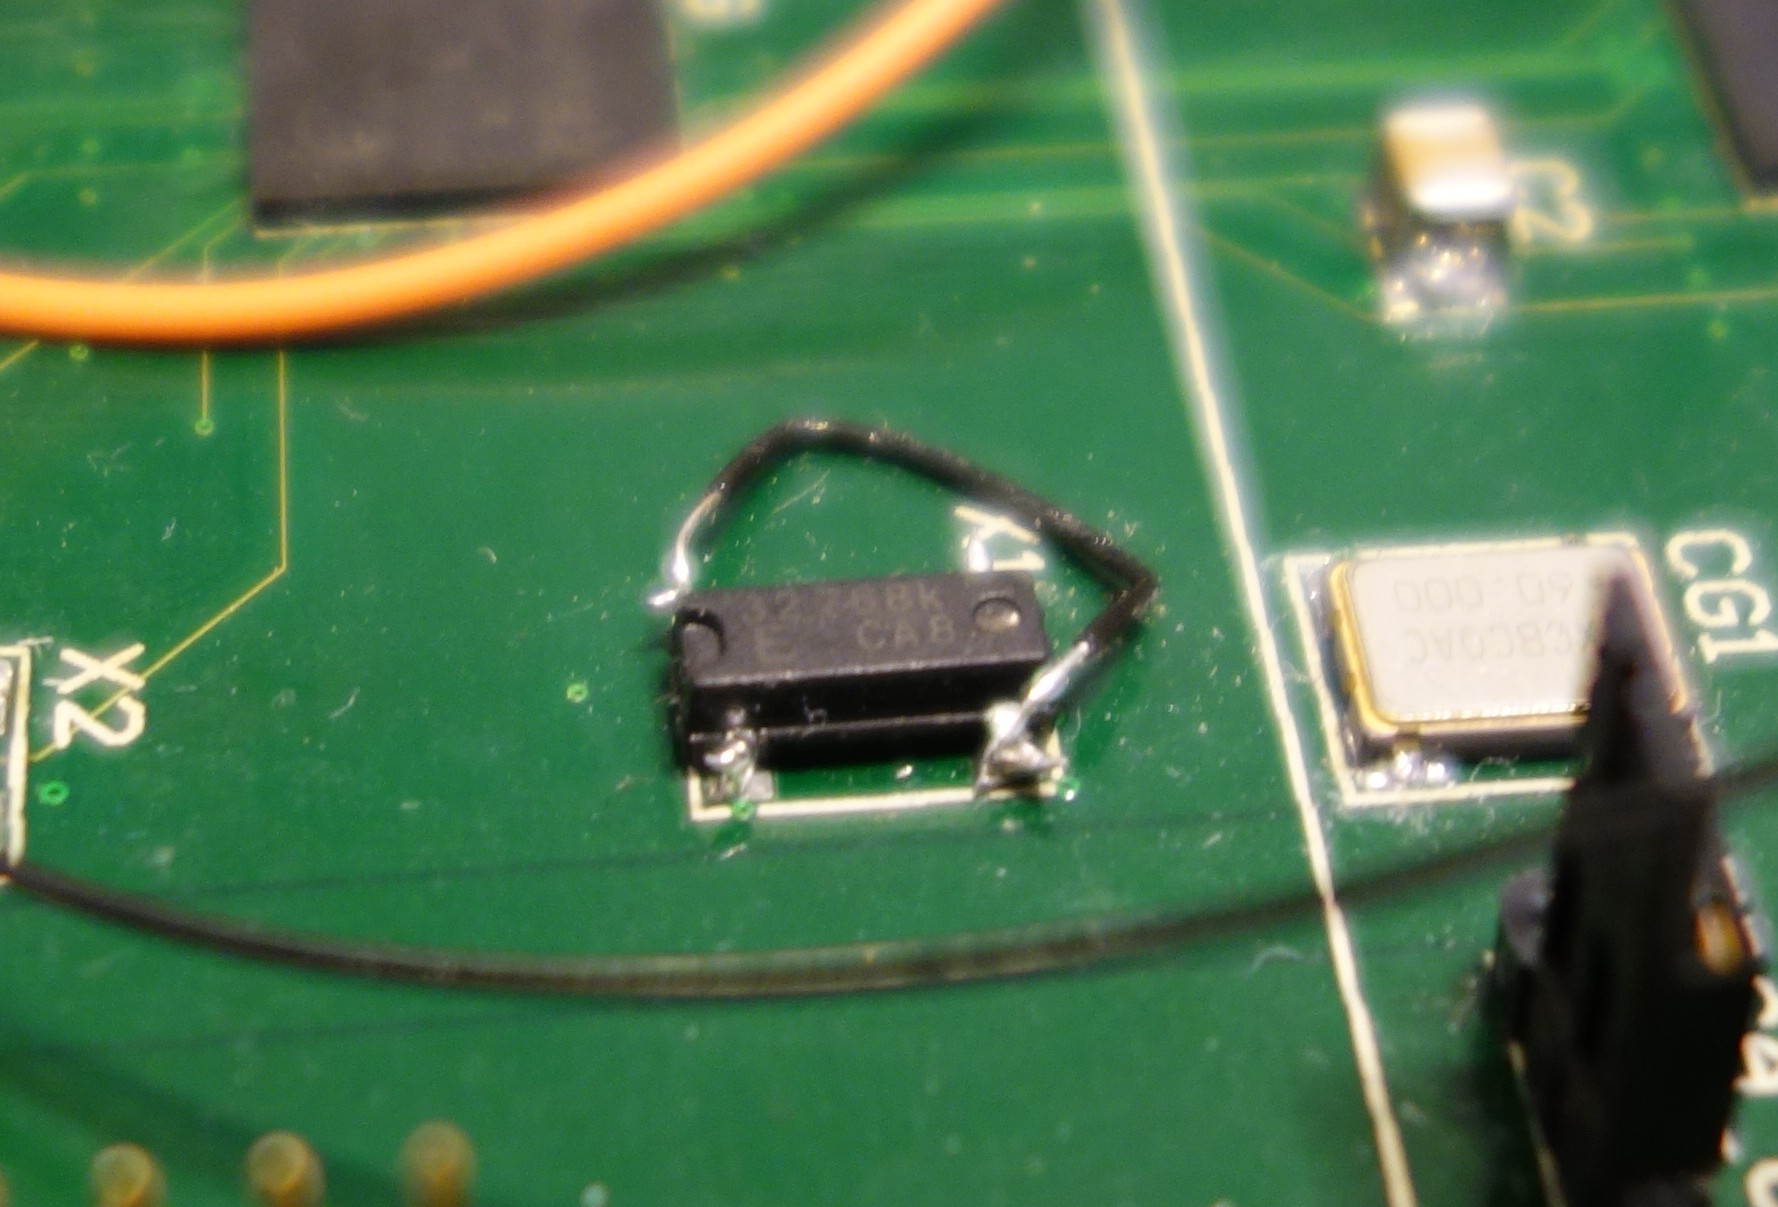
\includegraphics[scale=0.1]{figures/results/pcb/lfxtal}
    \caption{Low frequency crystal hack.}
    \label{fig:res:lfxtal}
\end{figure}



The linear regulator was slightly more advanced as pin 1 and 5, and 2, 3 and 4,
had been swapped. The solution was to solder six short patch cables on the pads
themselves, and then match the feet of the linear regulator with the right
cables. This resulted in the linear regulator being mounted about 1 cm above the
card.

\begin{figure}[H]
    \centering
    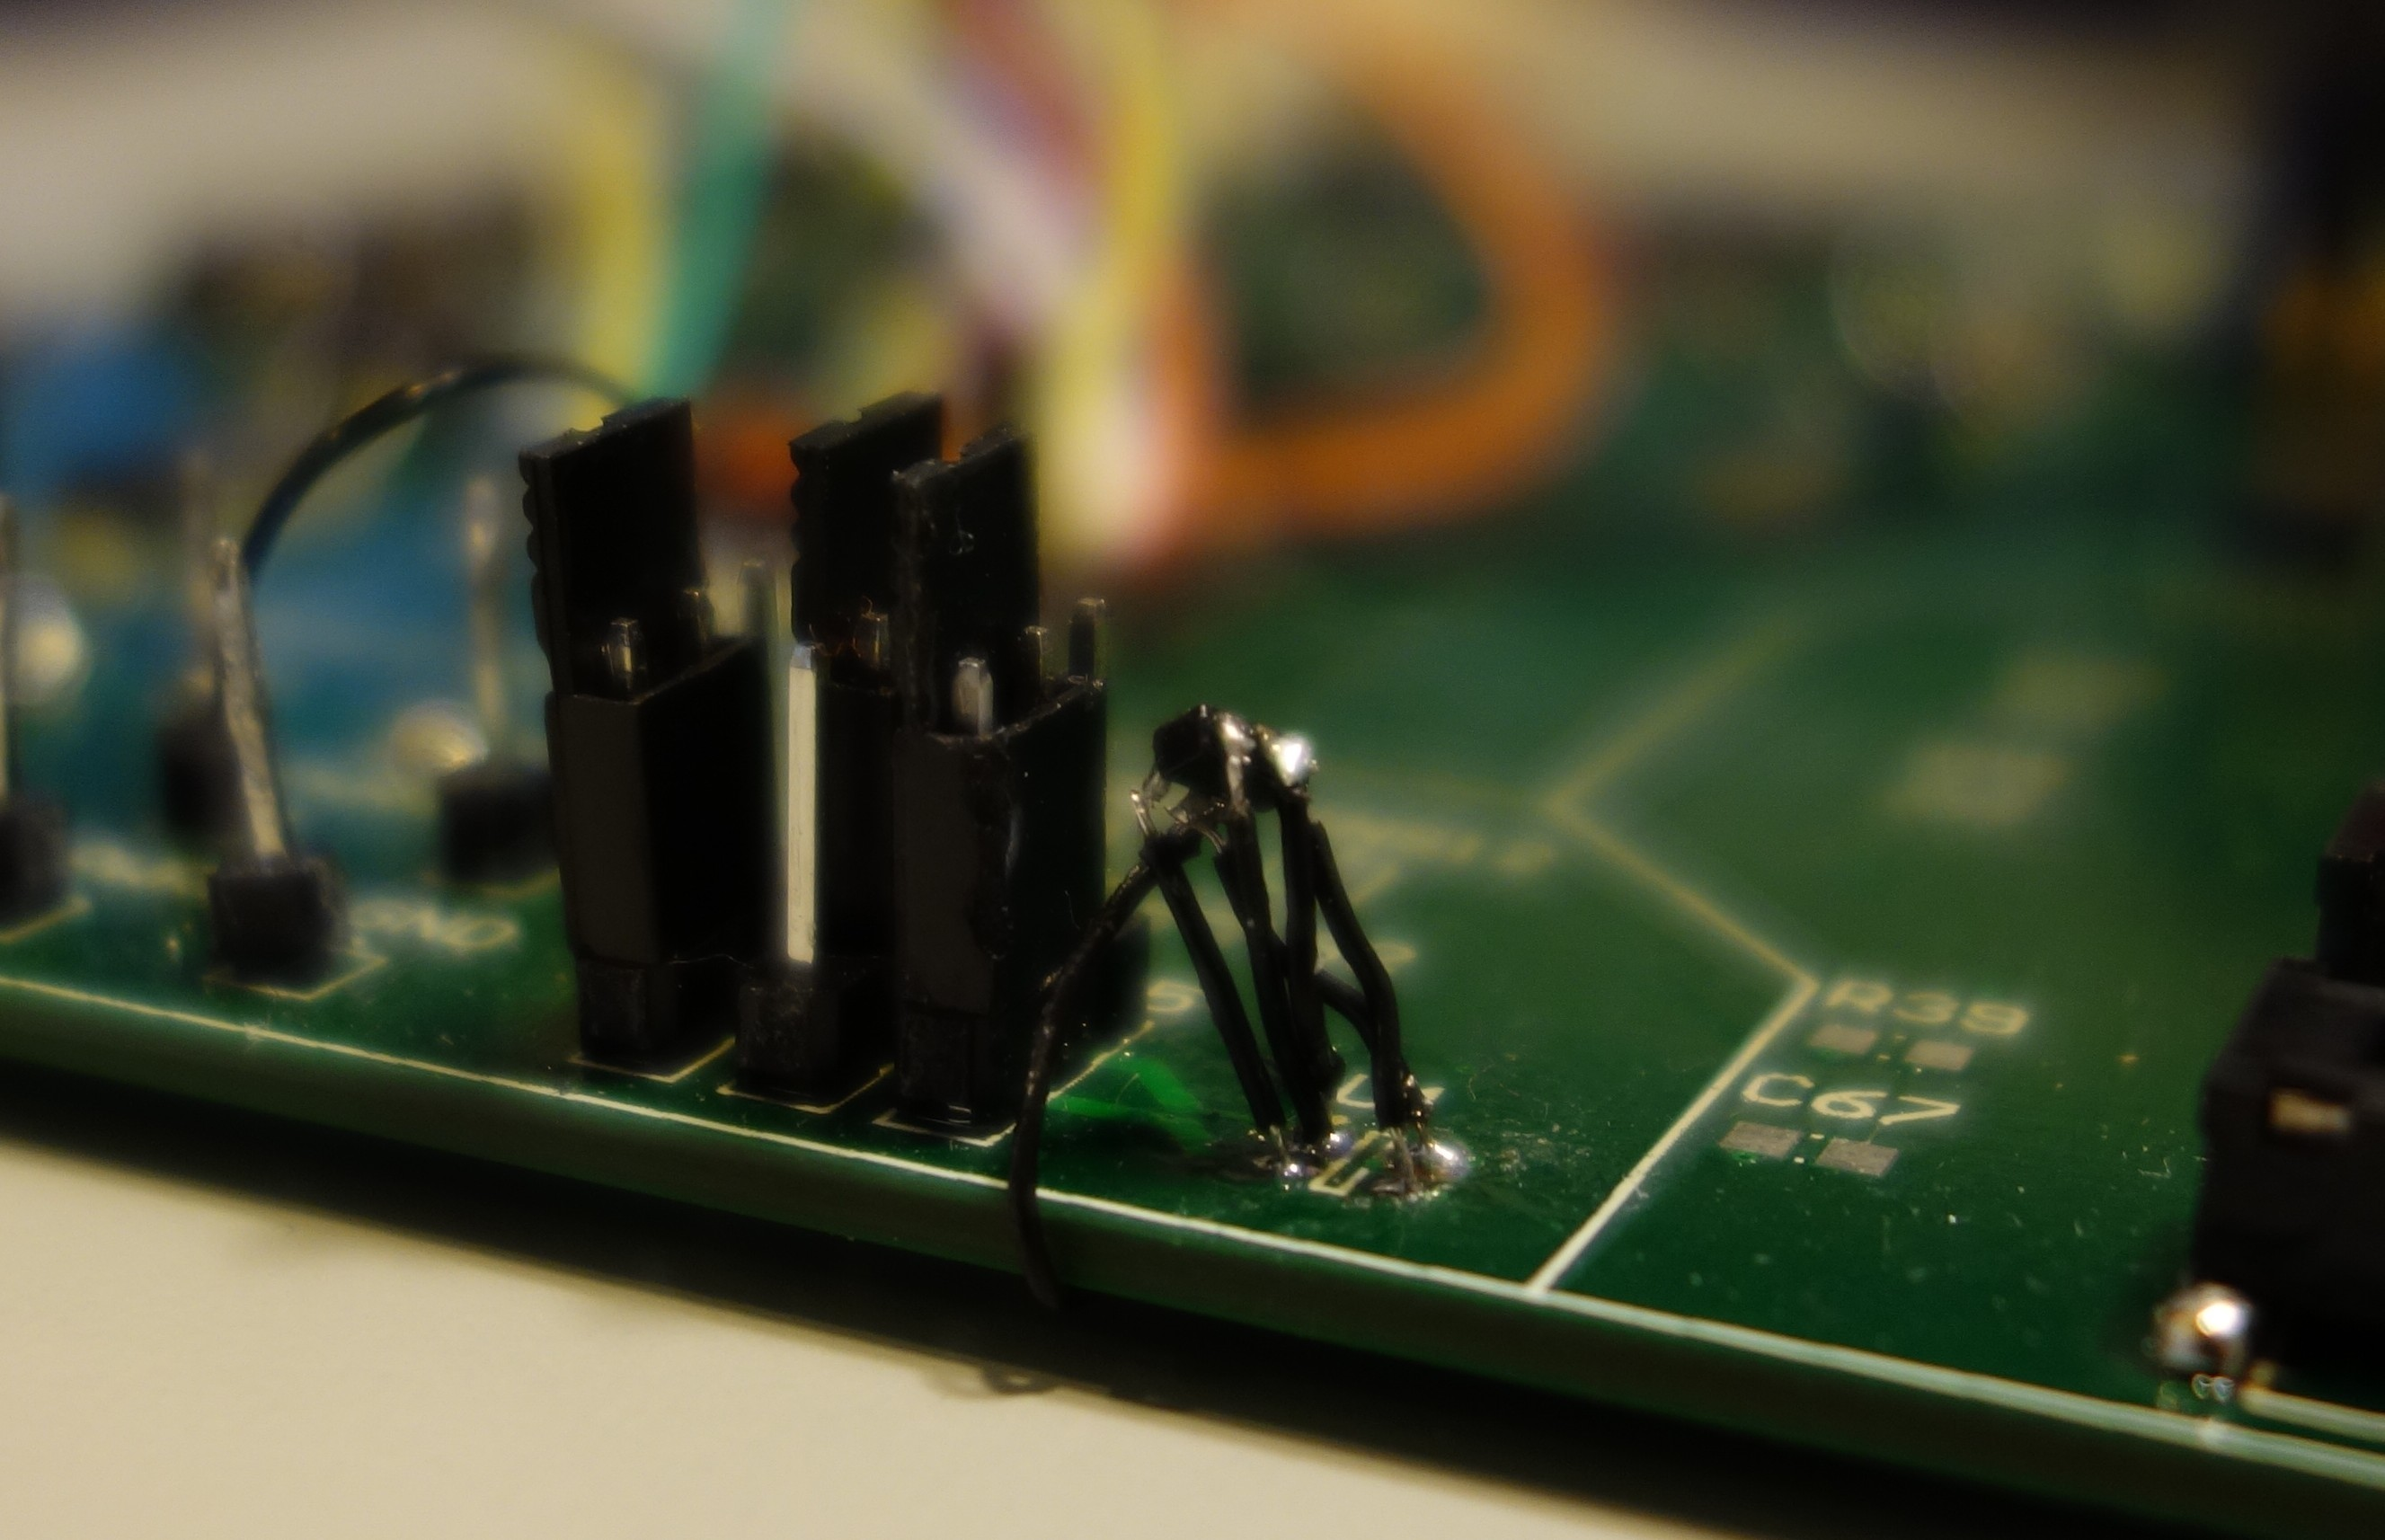
\includegraphics[scale=0.1]{figures/results/pcb/linear-regulator.jpg}
    \caption{Linear voltage regulator hack.}
    \label{fig:res:linreg}
\end{figure}



In addition, due to a typo in the schematic, the data lines of the EBI bus were
only connected to the MCU and external RAM, not to the FPGA. Again, this was
solved by patch cables between the external RAM's data pins and all available
FPGA GPIO pins. The result was a fully functional bus as was originally
intended, at the expense of all other I/O opportunities on the FPGA. All 12 GPIO
pins were used, as well as two buttons and two LED's, adding up to 16 bits.

% !TEX root = ../../../../report.tex
\subsubsection{Bus interface}

While not strictly a component, the databus is still an important part of
the PCB design. The MCU natively supports two bus interfaces, I2C and EBI,
of which the latter was used. This was done because I2C as a
serial bus has more limited bandwidth compared to the EBI, which
supports 16 bit words. The need for speed stems from the requirement of
streaming at least two audio streams live between the MCU and FPGA.
As an added bonus, the EBI bus is compatible with SRAM chip interfaces
which proved useful when including extra memory in the design.

In addition to the EBI bus there is a special control bus with a width
of 3 signals going between the MCU and FPGA. This bus is available for the
software and FPGA group to use as needed, for instance for interrupts or
other forms of synchronization and status signaling.


Finally, there was an actual connection error in the external RAM footprint.
One of the two chip select inputs, CS1, was suppose to be grounded, but had
mistakenly been connected to VCC33, resulting in the unit being stuck in off
mode. To solve this, the chip select pin was bent slightly upwards and then
connected with a patch cable to a GND pin nearby. However, due to the bus
workaround the SRAM was completely disabled and not used.


